 \documentclass{article}\usepackage[]{graphicx}\usepackage[]{color}
%% maxwidth is the original width if it is less than linewidth
%% otherwise use linewidth (to make sure the graphics do not exceed the margin)
\makeatletter
\def\maxwidth{ %
  \ifdim\Gin@nat@width>\linewidth
    \linewidth
  \else
    \Gin@nat@width
  \fi
}
\makeatother

\definecolor{fgcolor}{rgb}{0.345, 0.345, 0.345}
\newcommand{\hlnum}[1]{\textcolor[rgb]{0.686,0.059,0.569}{#1}}%
\newcommand{\hlstr}[1]{\textcolor[rgb]{0.192,0.494,0.8}{#1}}%
\newcommand{\hlcom}[1]{\textcolor[rgb]{0.678,0.584,0.686}{\textit{#1}}}%
\newcommand{\hlopt}[1]{\textcolor[rgb]{0,0,0}{#1}}%
\newcommand{\hlstd}[1]{\textcolor[rgb]{0.345,0.345,0.345}{#1}}%
\newcommand{\hlkwa}[1]{\textcolor[rgb]{0.161,0.373,0.58}{\textbf{#1}}}%
\newcommand{\hlkwb}[1]{\textcolor[rgb]{0.69,0.353,0.396}{#1}}%
\newcommand{\hlkwc}[1]{\textcolor[rgb]{0.333,0.667,0.333}{#1}}%
\newcommand{\hlkwd}[1]{\textcolor[rgb]{0.737,0.353,0.396}{\textbf{#1}}}%

\usepackage{framed}
\makeatletter
\newenvironment{kframe}{%
 \def\at@end@of@kframe{}%
 \ifinner\ifhmode%
  \def\at@end@of@kframe{\end{minipage}}%
  \begin{minipage}{\columnwidth}%
 \fi\fi%
 \def\FrameCommand##1{\hskip\@totalleftmargin \hskip-\fboxsep
 \colorbox{shadecolor}{##1}\hskip-\fboxsep
     % There is no \\@totalrightmargin, so:
     \hskip-\linewidth \hskip-\@totalleftmargin \hskip\columnwidth}%
 \MakeFramed {\advance\hsize-\width
   \@totalleftmargin\z@ \linewidth\hsize
   \@setminipage}}%
 {\par\unskip\endMakeFramed%
 \at@end@of@kframe}
\makeatother

\definecolor{shadecolor}{rgb}{.97, .97, .97}
\definecolor{messagecolor}{rgb}{0, 0, 0}
\definecolor{warningcolor}{rgb}{1, 0, 1}
\definecolor{errorcolor}{rgb}{1, 0, 0}
\newenvironment{knitrout}{}{} % an empty environment to be redefined in TeX

\usepackage{alltt}
\usepackage[margin=1in]{geometry}
%\VignetteIndexEntry{How to use RSGHB}

\usepackage{url}
\makeatletter
\def\url@leostyle{%
  \@ifundefined{selectfont}{\def\UrlFont{\sf}}{\def\UrlFont{\small\ttfamily}}}
\makeatother
\urlstyle{leo}
\IfFileExists{upquote.sty}{\usepackage{upquote}}{}
\begin{document}

\title{How to use RSGHB}
\author{Jeffrey Dumont, Jeff Keller}
\date{June 2015}
\maketitle
\abstract{This vignette describes the process for specifying, estimating and analyzing the output of a choice model with RSGHB. Two case studies with different model structures are used as examples. The synthetic choice data set \emph{choicedata} used in this document is included in the RSGHB package or can be downloaded from the RSGHB github page: \url{https://github.com/jeffdumont/RSGHB}}

\begin{center}
\line(1,0){400}
\end{center}

\section*{RSGHB Code Structure}

The code typically needed for running an RSGHB model can be broken into five main sections and the examples that follow are organized in this manner.

\begin{enumerate}
     \item Setup and Data Preparation
     \item Defining the Likelihood Function
     \item Model Controls and Settings
     \item Model Estimation
     \item The Output
\end{enumerate}

Previous versions of RSGHB produced a series of CSV files as output. Newer versions of RSGHB produce a model object of class \emph{RSGHB} that can be operated on directly. However, the old behavior can be restored by using the \emph{writeModel} function or by setting the \emph{writeModel} argument in \emph{doHB} to \emph{TRUE}.

\section*{EXAMPLE 1: MNL Model with Fixed Parameters}

In this section, the code for estimating a multinomial logit (MNL) model with fixed (non-random) parameters is explained. The data set for this example is composed of synthetic individuals that were presented with a choice between two travel alternatives - one that is toll-free and one that had a toll but also had a faster travel time. Each of 1,138 individuals was presented with a panel of 9 choice tasks.

\subsection*{Setup and Data Preparation}

\begin{knitrout}
\definecolor{shadecolor}{rgb}{0.969, 0.969, 0.969}\color{fgcolor}\begin{kframe}
\begin{alltt}
\hlkwd{library}\hlstd{(RSGHB)}

\hlcom{# Load example data}
\hlkwd{data}\hlstd{(choicedata)}

\hlcom{# This data set is organized as one row per choice observation. This isn't necessary }
\hlcom{# but it does make writing the likelihood function straightforward.}
\hlkwd{head}\hlstd{(choicedata)}
\end{alltt}
\begin{verbatim}
##     ID thecount tt1 tt2 toll2 asc1 Choice
## 1 8738        1  60  51  1.25    1      1
## 2 8738        2  60  51  0.75    1      1
## 3 8738        3  63  59  0.50    1      2
## 4 8738        4  60  54  0.75    1      1
## 5 8738        5  60  54  0.50    1      2
## 6 8738        6  63  54  0.75    1      1
\end{verbatim}
\begin{alltt}
\hlcom{# Any variables or transformations of variables from the choicedata data.frame that are}
\hlcom{# needed for evaluating the likelihood function can be extracted as a series of vectors}
\hlcom{# for convenience (e.g., TT1, TT2, TOLL2). Alternatively, the likelihood function could}
\hlcom{# refer to the choicedata data.frame directly. In this example, each alternative is}
\hlcom{# defined by travel times and toll costs.}
\hlstd{TT1}   \hlkwb{<-} \hlstd{choicedata}\hlopt{$}\hlstd{tt1}
\hlstd{TT2}   \hlkwb{<-} \hlstd{choicedata}\hlopt{$}\hlstd{tt2}
\hlstd{TOLL2} \hlkwb{<-} \hlstd{choicedata}\hlopt{$}\hlstd{toll2}

\hlcom{# Similarly for the vectors of choices. Note that in this example, there are only two }
\hlcom{# alternatives. Dummying coding the choice vector is not necessary but again makes}
\hlcom{# writing the likelihood function straightforward.}
\hlstd{choice1} \hlkwb{<-} \hlstd{(choicedata}\hlopt{$}\hlstd{Choice}\hlopt{==}\hlnum{1}\hlstd{)}
\hlstd{choice2} \hlkwb{<-} \hlstd{(choicedata}\hlopt{$}\hlstd{Choice}\hlopt{==}\hlnum{2}\hlstd{)}

\hlcom{# Frequency of choices}
\hlkwd{table}\hlstd{(choicedata}\hlopt{$}\hlstd{Choice)}
\end{alltt}
\begin{verbatim}
## 
##    1    2 
## 6682 3560
\end{verbatim}
\end{kframe}
\end{knitrout}

\subsection*{Defining the Likelihood Function}

The estimation routine expects a user-specified \emph{likelihood} function that accepts two arguments, \emph{fc} and \emph{b}, that, in concert with the choice data, returns a vector of probabilities of length equal to the number of total choice tasks across all respondents. With 1,138 respondents and 9 choice tasks each, the \emph{likelihood} function should return a vector of length 1,138*9=10,242 in this case.

The \emph{fc} argument is a vector of fixed coefficients (they do not vary across individuals). The \emph{b} argument is a matrix of individual coefficients which are generated from the random coefficients in the model. The \emph{b} matrix is discussed in more detail in Example 2.

It is important to note that the structure of the \emph{likelihood} function and choice data set is arbitrary, and completely up to the user, so long as the \emph{likelihood} function accepts \emph{fc} and \emph{b} as arguments and returns a vector of probabilities of appropriate length. However, the \emph{likelihood} function is the most computationally taxing part of the estimation process, so coding this function efficiently is essential to reducing the run time of the model.

\begin{knitrout}
\definecolor{shadecolor}{rgb}{0.969, 0.969, 0.969}\color{fgcolor}\begin{kframe}
\begin{alltt}
\hlcom{# The likelihood function}
\hlstd{likelihood} \hlkwb{<-} \hlkwa{function}\hlstd{(}\hlkwc{fc}\hlstd{,} \hlkwc{b}\hlstd{) \{}

  \hlcom{# Assign fixed parameters to named variables for convenience    }
  \hlstd{cc} \hlkwb{<-} \hlnum{1}
  \hlstd{ASC1}  \hlkwb{<-} \hlstd{fc[cc]; cc} \hlkwb{<-} \hlstd{cc} \hlopt{+} \hlnum{1}
  \hlstd{Btime} \hlkwb{<-} \hlstd{fc[cc]; cc} \hlkwb{<-} \hlstd{cc} \hlopt{+} \hlnum{1}
  \hlstd{Btoll} \hlkwb{<-} \hlstd{fc[cc]; cc} \hlkwb{<-} \hlstd{cc} \hlopt{+} \hlnum{1}

  \hlcom{# Utility functions}
  \hlstd{v1} \hlkwb{<-} \hlstd{ASC1} \hlopt{+} \hlstd{Btime} \hlopt{*} \hlstd{TT1}
  \hlstd{v2} \hlkwb{<-}        \hlstd{Btime} \hlopt{*} \hlstd{TT2} \hlopt{+} \hlstd{Btoll} \hlopt{*} \hlstd{TOLL2}

  \hlcom{# MNL probability statement}
  \hlstd{p}  \hlkwb{<-} \hlstd{(}\hlkwd{exp}\hlstd{(v1)} \hlopt{*} \hlstd{choice1} \hlopt{+} \hlkwd{exp}\hlstd{(v2)} \hlopt{*} \hlstd{choice2)} \hlopt{/} \hlstd{(}\hlkwd{exp}\hlstd{(v1)} \hlopt{+} \hlkwd{exp}\hlstd{(v2))}

  \hlkwd{return}\hlstd{(p)}
\hlstd{\}}
\end{alltt}
\end{kframe}
\end{knitrout}

\subsection*{Model Controls and Settings}

There are a number of options and settings for controlling the model estimation process. Please see the help file for \emph{doHB} for more details. Note that most controls have default values and do not need to be directly specified if the default is acceptable.

\begin{knitrout}
\definecolor{shadecolor}{rgb}{0.969, 0.969, 0.969}\color{fgcolor}\begin{kframe}
\begin{alltt}
\hlcom{### Setting control list for estimation (see ?doHB for more estimation options)}

\hlcom{# The model name/description}
\hlstd{modelname} \hlkwb{<-} \hlstr{"MNL"}

\hlcom{# gVarNamesFixed contains the names for the fixed (non-random) variables in the model}
\hlcom{# These will be used in the output and also when displaying iteration detail to }
\hlcom{# the screen}
\hlstd{gVarNamesFixed} \hlkwb{<-} \hlkwd{c}\hlstd{(}\hlstr{"ASC1"}\hlstd{,} \hlstr{"BTime"}\hlstd{,} \hlstr{"BCost"}\hlstd{)}

\hlcom{# FC contains the starting values for the fixed coefficients}
\hlstd{FC} \hlkwb{<-} \hlkwd{c}\hlstd{(}\hlnum{0}\hlstd{,} \hlnum{0}\hlstd{,} \hlnum{0}\hlstd{)}

\hlcom{# gNCREP contains the number of iterations to use prior to convergence}
\hlstd{gNCREP} \hlkwb{<-} \hlnum{2500}
\hlcom{# gNEREP contains the number of iterations to keep for averaging after convergence }
\hlcom{# has been reached}
\hlstd{gNEREP} \hlkwb{<-} \hlnum{2500}
\hlcom{# gNSKIP contains the number of iterations between retaining draws for averaging}
\hlstd{gNSKIP} \hlkwb{<-} \hlnum{1}
\hlcom{# gINFOSKIP controls how frequently to print info about the iteration process}
\hlstd{gINFOSKIP} \hlkwb{<-} \hlnum{10}
\hlcom{# gSeed ensures reproducible results}
\hlstd{gSeed} \hlkwb{<-} \hlnum{1987}

\hlcom{# To simplify the doHB function call, all of the control arguments are placed in }
\hlcom{# a single list that can be passed directly to doHB}
\hlstd{control} \hlkwb{<-} \hlkwd{list}\hlstd{(}\hlkwc{modelname} \hlstd{= modelname,}
                \hlkwc{gVarNamesFixed} \hlstd{= gVarNamesFixed,}
                \hlkwc{FC} \hlstd{= FC,}
                \hlkwc{gNCREP} \hlstd{= gNCREP,}
                \hlkwc{gNEREP} \hlstd{= gNEREP,}
                \hlkwc{gNSKIP} \hlstd{= gNSKIP,}
                \hlkwc{gINFOSKIP} \hlstd{= gINFOSKIP,}
                \hlkwc{gSeed} \hlstd{= gSeed)}
\end{alltt}
\end{kframe}
\end{knitrout}

\subsection*{Model Estimation}

To start the model estimation process, the analyst passes the \emph{likelihood} function, \emph{choicedata} data.frame, and the \emph{control} list to the \emph{doHB} function.

\begin{verbatim}
model <- doHB(likelihood, choicedata, control)
\end{verbatim}



Note that the only requirement of the \emph{choicedata} data.frame is that it contains a column \emph{ID} which identifies the individuals associated with the vector of probabilities returned by the \emph{likelihood} function.

The \emph{doHB} function will perform a series of diagnostic tests on the model inputs to catch common errors in model setup. It also provides basic summary statistics of the choice data and model. Before estimation begins, an optional confirmation prompt allows the user to cancel the model estimation if needed.

\begin{figure}
\caption{Plotting of the Markov Chains during estimation}
\centering
\includegraphics[scale=0.50]{MNL_MarkovChains.png}
\label{MarkovChain}
\end{figure}

During estimation, current estimates of the Markov Chains will be plotted to the screen. This plot is updated based on the control parameter \emph{gINFOSKIP} (Figure \ref{MarkovChain}). In addition, numerical iteration details are provided in the R Console. Printing and plotting during model estimation takes time, so increasing \emph{gINFOSKIP} will reduce estimation time.

\subsection*{The Output}

The \emph{doHB} function returns a model object of class \emph{RSGHB}. See \emph{?doHB} for a detailed description of the components of an \emph{RSGHB} class model object.

In addition to the modeling controls and settings, the model object includes an \emph{iter.detail} component that contains model statistics at every \emph{gINFOSKIP}th iteration. These can be used to assess whether the model has converged. This model has only fixed parameters, so only the Log-Likelihood, Root-Likelihood (RLH), and Acceptance Rate for the fixed parameters are meaningful.

\begin{knitrout}
\definecolor{shadecolor}{rgb}{0.969, 0.969, 0.969}\color{fgcolor}\begin{kframe}
\begin{alltt}
\hlcom{# Model iteration details}
\hlkwd{head}\hlstd{(model[[}\hlstr{"iter.detail"}\hlstd{]])}
\end{alltt}
\begin{verbatim}
##   Iteration Log-Likelihood       RLH Parameter RMS Avg. Variance
## 2         1      -7099.213 0.5000000            NA            NA
## 3        10      -6973.993 0.5062999            NA            NA
## 4        20      -6834.960 0.5148242            NA            NA
## 5        30      -6798.906 0.5166043            NA            NA
## 6        40      -6787.540 0.5174368            NA            NA
## 7        50      -6760.764 0.5187301            NA            NA
##   Acceptance Rate (Fixed) Acceptance Rate (Normal)
## 2                       0                       NA
## 3                       0                       NA
## 4                       0                       NA
## 5                       0                       NA
## 6                       0                       NA
## 7                       0                       NA
\end{verbatim}
\end{kframe}
\end{knitrout}

The RSGHB plot method visualizes these model statistics conveniently.

\begin{knitrout}
\definecolor{shadecolor}{rgb}{0.969, 0.969, 0.969}\color{fgcolor}\begin{kframe}
\begin{alltt}
\hlcom{# Plot model statistics}
\hlkwd{plot}\hlstd{(model)}
\end{alltt}
\end{kframe}
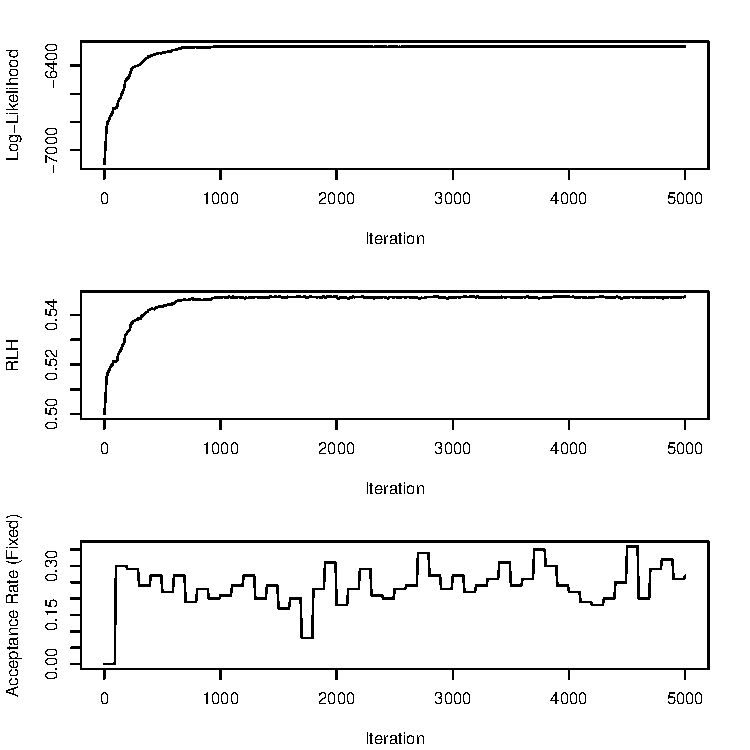
\includegraphics[width=\maxwidth]{figure/unnamed-chunk-6-1} 

\end{knitrout}

Similarly, supplying the \emph{type} argument to the plot method will plot the fixed parameter estimates, which are contained in the \emph{F} component of the model object.

\begin{knitrout}
\definecolor{shadecolor}{rgb}{0.969, 0.969, 0.969}\color{fgcolor}\begin{kframe}
\begin{alltt}
\hlcom{# Plot parameter estimates (see ?plot.RSGHB for more uses)}
\hlkwd{plot}\hlstd{(model,} \hlkwc{type} \hlstd{=} \hlstr{"F"}\hlstd{)}
\end{alltt}
\end{kframe}
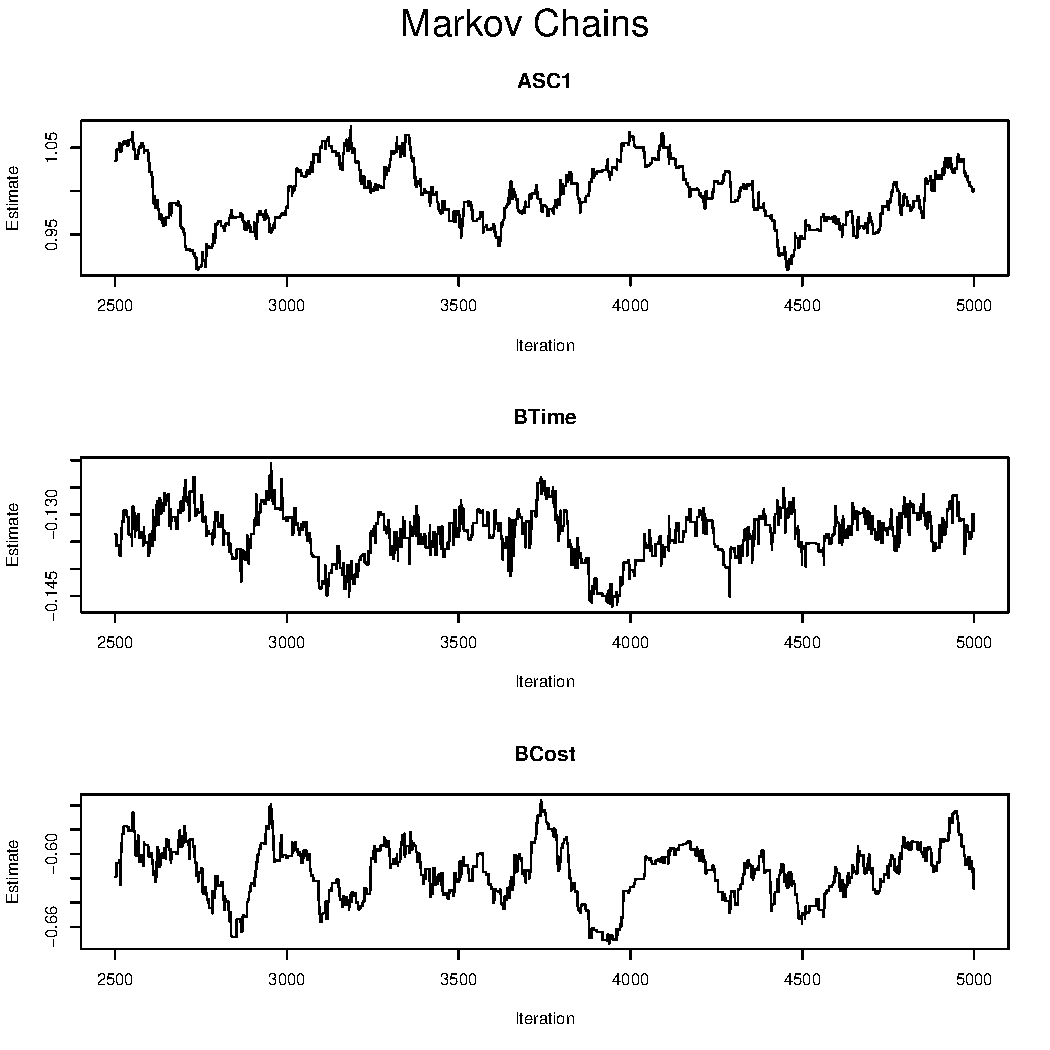
\includegraphics[width=\maxwidth]{figure/unnamed-chunk-7-1} 

\end{knitrout}

\section*{EXAMPLE 2: MNL Model with Random Coefficients}

In this section, we expand on the model estimated in Example 1 by allowing the coefficients to vary across the individuals in our dataset. This type of model is referred to by many names - Random Coefficients Logit, Random Parameters Logit or Mixed Logit. 

\subsection*{Setup and Data Preparation}

The setup and data preparation are identical to Example 1.

\subsection*{Defining the Likelihood Function}

To introduce random effects into the model, the \emph{b} matrix is used in place of the \emph{fc} vector in the coding of the \emph{likelihood} function. The \emph{b} matrix contains the individual conditionals for the sample-level random coefficients. The matrix \emph{b} has one row per choice task (associated with the vector of probabilities returned by the \emph{likelihood} function) and one column for each of the random parameters.

\begin{knitrout}
\definecolor{shadecolor}{rgb}{0.969, 0.969, 0.969}\color{fgcolor}\begin{kframe}
\begin{alltt}
\hlstd{likelihood} \hlkwb{<-} \hlkwa{function}\hlstd{(}\hlkwc{fc}\hlstd{,} \hlkwc{b}\hlstd{) \{}

     \hlcom{# Note that the fc argument is still supplied, but is unused}

     \hlcom{# Using b instead of fc is the only change}
     \hlstd{cc}     \hlkwb{<-} \hlnum{1}
     \hlstd{ASC1}   \hlkwb{<-} \hlstd{b[, cc]; cc} \hlkwb{<-} \hlstd{cc} \hlopt{+} \hlnum{1}
     \hlstd{Btime}  \hlkwb{<-} \hlstd{b[, cc]; cc} \hlkwb{<-} \hlstd{cc} \hlopt{+} \hlnum{1}
     \hlstd{Btoll}  \hlkwb{<-} \hlstd{b[, cc]; cc} \hlkwb{<-} \hlstd{cc} \hlopt{+} \hlnum{1}

     \hlcom{# Utility functions}
     \hlstd{v1} \hlkwb{<-} \hlstd{ASC1} \hlopt{+} \hlstd{Btime} \hlopt{*} \hlstd{TT1}
     \hlstd{v2} \hlkwb{<-}        \hlstd{Btime} \hlopt{*} \hlstd{TT2} \hlopt{+} \hlstd{Btoll} \hlopt{*} \hlstd{TOLL2}

     \hlcom{# MNL probability statement}
     \hlstd{p}  \hlkwb{<-} \hlstd{(}\hlkwd{exp}\hlstd{(v1)} \hlopt{*} \hlstd{choice1} \hlopt{+} \hlkwd{exp}\hlstd{(v2)} \hlopt{*} \hlstd{choice2)} \hlopt{/} \hlstd{(}\hlkwd{exp}\hlstd{(v1)} \hlopt{+} \hlkwd{exp}\hlstd{(v2))}

     \hlkwd{return}\hlstd{(p)}
\hlstd{\}}
\end{alltt}
\end{kframe}
\end{knitrout}

\subsection*{Model Controls and Settings}

A few more controls can be supplied to the \emph{doHB} function when random parameters are to be estimated.

\begin{knitrout}
\definecolor{shadecolor}{rgb}{0.969, 0.969, 0.969}\color{fgcolor}\begin{kframe}
\begin{alltt}
\hlcom{### Setting control list for estimation (see ?doHB for more estimation options)}

\hlcom{# The model name/description}
\hlstd{modelname} \hlkwb{<-} \hlstr{"MMNL"}

\hlcom{# gVarNamesNormal provides names for the random parameters in the same way}
\hlcom{# gVarNamesFixed does for the fixed parameters}
\hlstd{gVarNamesNormal} \hlkwb{<-} \hlkwd{c}\hlstd{(}\hlstr{"ASC1"}\hlstd{,}\hlstr{"BTime"}\hlstd{,}\hlstr{"BCost"}\hlstd{)}

\hlcom{# svN contains the starting values for the means of the normal distributions for each }
\hlcom{# of the random parameters}
\hlstd{svN} \hlkwb{<-} \hlkwd{c}\hlstd{(}\hlnum{0}\hlstd{,} \hlnum{0}\hlstd{,} \hlnum{0}\hlstd{)}

\hlcom{# gDIST specifies the type of continuous distribution to use for the random parameters}
\hlcom{# gDIST must have an entry for each value in gVarNamesNormal}
\hlcom{# The options are:}
\hlcom{# 1. normal}
\hlcom{# 2. log-nomal}
\hlcom{# 3. negative log-normal}
\hlcom{# 4. normal with all values below zero massed at zero}
\hlcom{# 5. normal with all values greater than zero massed at zero}
\hlcom{# 6. Johnson SB with a specified min and max}

\hlcom{# In this example, normal distributions are used for all 3 parameters}
\hlstd{gDIST} \hlkwb{<-} \hlkwd{c}\hlstd{(}\hlnum{1}\hlstd{,} \hlnum{1}\hlstd{,} \hlnum{1}\hlstd{)}

\hlcom{# gNCREP contains the number of iterations to use prior to convergence}
\hlstd{gNCREP} \hlkwb{<-} \hlnum{2500}
\hlcom{# gNEREP contains the number of iterations to keep for averaging after convergence }
\hlcom{# has been reached}
\hlstd{gNEREP} \hlkwb{<-} \hlnum{2500}
\hlcom{# gNSKIP contains the number of iterations between retaining draws for averaging}
\hlstd{gNSKIP} \hlkwb{<-} \hlnum{1}
\hlcom{# gINFOSKIP controls how frequently to print info about the iteration process}
\hlstd{gINFOSKIP} \hlkwb{<-} \hlnum{10}
\hlcom{# gSeed ensures reproducible results}
\hlstd{gSeed} \hlkwb{<-} \hlnum{1987}

\hlcom{# To simplify the doHB function call, all of the control parameters are placed in}
\hlcom{# a single list that can be passed directly to doHB}
\hlstd{control} \hlkwb{<-} \hlkwd{list}\hlstd{(}\hlkwc{modelname} \hlstd{= modelname,}
                \hlkwc{gVarNamesNormal} \hlstd{= gVarNamesNormal,}
                \hlkwc{gDIST} \hlstd{= gDIST,}
                \hlkwc{svN} \hlstd{= svN,}
                \hlkwc{gNCREP} \hlstd{= gNCREP,}
                \hlkwc{gNEREP} \hlstd{= gNEREP,}
                \hlkwc{gNSKIP} \hlstd{= gNSKIP,}
                \hlkwc{gINFOSKIP} \hlstd{= gINFOSKIP,}
                \hlkwc{gSeed} \hlstd{= gSeed)}
\end{alltt}
\end{kframe}
\end{knitrout}

\subsection*{Model Estimation}

As in Example 1, the model estimation process is initiated with the analyst supplying the \emph{likelihood} function, \emph{choicedata} data.frame, and the \emph{control} list to the \emph{doHB} function.

\begin{verbatim}
model <- doHB(likelihood, choicedata, control)
\end{verbatim}



In this model, the Markov Chain values plotted represent the means of the underlying normals for the random parameters (Figure \ref{MarkovChain2}).

\begin{figure}
\caption{Plotting of the Markov Chains during estimation}
\centering
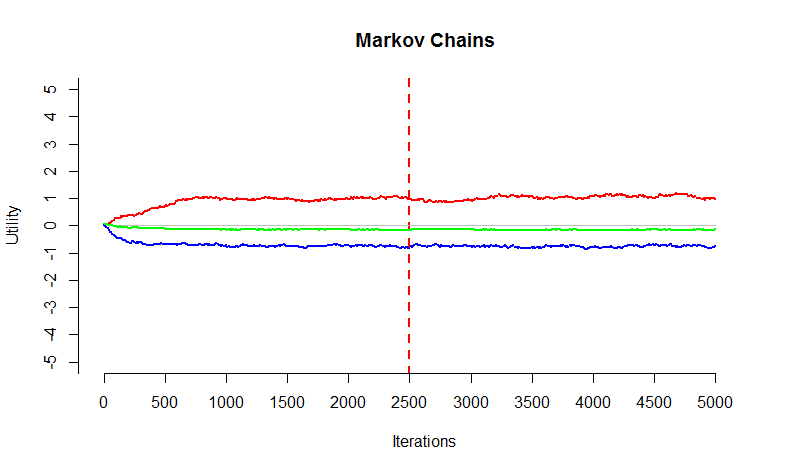
\includegraphics[scale=0.50]{MMNL_MarkovChains.png}
\label{MarkovChain2}
\end{figure}

\subsection*{The Output}

The \emph{RSGHB} model object has more components in the case of a random or mixed effects model.

The \emph{iter.detail} component now contains the additional model statistics: Parameter Root Mean Square (RMS) and Average Variance at each stored iteration.

\begin{knitrout}
\definecolor{shadecolor}{rgb}{0.969, 0.969, 0.969}\color{fgcolor}\begin{kframe}
\begin{alltt}
\hlcom{# Model iteration details}
\hlkwd{head}\hlstd{(model[[}\hlstr{"iter.detail"}\hlstd{]])}
\end{alltt}
\begin{verbatim}
##   Iteration Log-Likelihood       RLH Parameter RMS Avg. Variance
## 2         1      -6875.096 0.5138458     0.1922419    0.03770582
## 3        10      -6530.749 0.5339567     0.2072798    0.04383990
## 4        20      -6408.916 0.5408803     0.2142815    0.04904044
## 5        30      -6348.262 0.5436143     0.2219182    0.05375706
## 6        40      -6286.665 0.5465279     0.2487251    0.07010541
## 7        50      -6294.444 0.5462534     0.2610000    0.07945012
##   Acceptance Rate (Fixed) Acceptance Rate (Normal)
## 2                      NA                0.2390158
## 3                      NA                0.6485062
## 4                      NA                0.4753954
## 5                      NA                0.3014060
## 6                      NA                0.2970123
## 7                      NA                0.2943761
\end{verbatim}
\begin{alltt}
\hlcom{# Plot model statistics}
\hlkwd{plot}\hlstd{(model)}
\end{alltt}
\end{kframe}
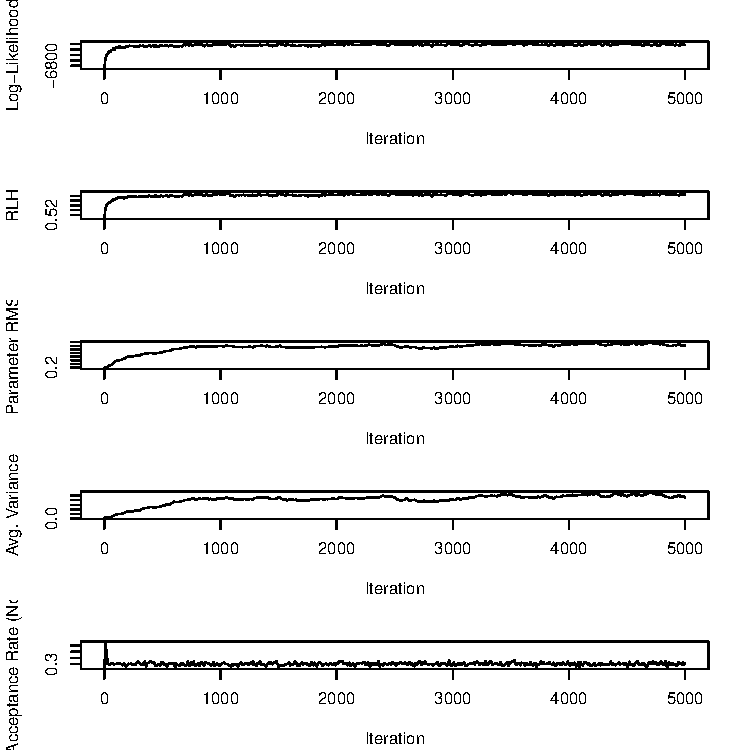
\includegraphics[width=\maxwidth]{figure/unnamed-chunk-11-1} 

\end{knitrout}

The \emph{A} component contains the sample-level means of the underlying normal. These can be plotted with the plot method.

\begin{knitrout}
\definecolor{shadecolor}{rgb}{0.969, 0.969, 0.969}\color{fgcolor}\begin{kframe}
\begin{alltt}
\hlcom{# Sample-level means}
\hlkwd{head}\hlstd{(model[[}\hlstr{"A"}\hlstd{]])}
\end{alltt}
\begin{verbatim}
##      iteration      ASC1      BTime      BCost
## [1,]      2501 0.9621848 -0.1545391 -0.8139106
## [2,]      2502 0.9545125 -0.1551021 -0.8220994
## [3,]      2503 0.9609168 -0.1579467 -0.8365826
## [4,]      2504 0.9566381 -0.1483454 -0.8112167
## [5,]      2505 0.9680402 -0.1513544 -0.7950746
## [6,]      2506 0.9622336 -0.1548498 -0.8074830
\end{verbatim}
\begin{alltt}
\hlcom{# Plot sample-level means}
\hlkwd{plot}\hlstd{(model,} \hlkwc{type} \hlstd{=} \hlstr{"A"}\hlstd{)}
\end{alltt}
\end{kframe}
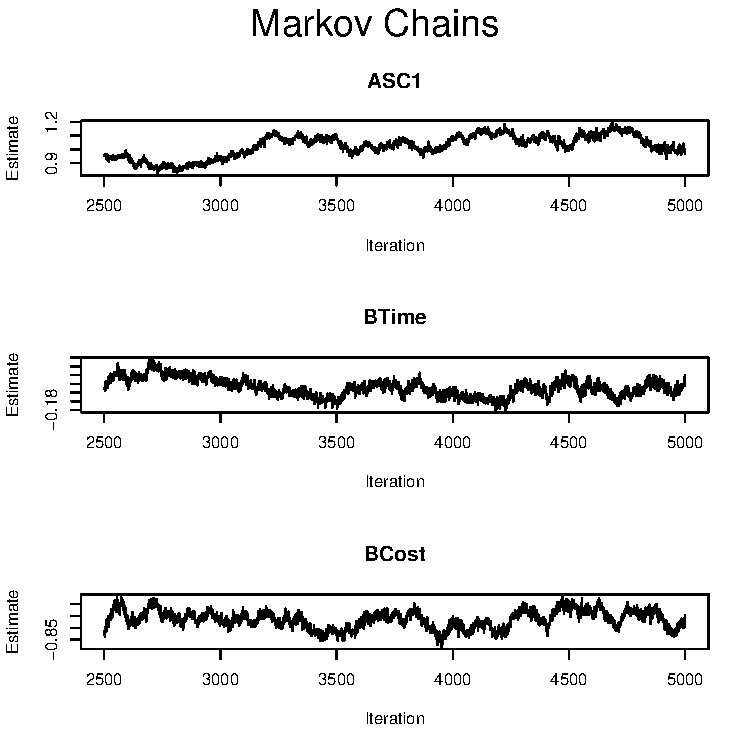
\includegraphics[width=\maxwidth]{figure/unnamed-chunk-12-1} 

\end{knitrout}

The \emph{B} component contains the average, across iterations, of the individual level draws for the underlying normals for the random parameters. The \emph{Bsd} component provides the standard deviations of those individual draws.

\begin{knitrout}
\definecolor{shadecolor}{rgb}{0.969, 0.969, 0.969}\color{fgcolor}\begin{kframe}
\begin{alltt}
\hlcom{# Average individual-level draws}
\hlkwd{head}\hlstd{(model[[}\hlstr{"B"}\hlstd{]])}
\end{alltt}
\begin{verbatim}
##      Respondent      ASC1       BTime      BCost
## [1,]       8738 1.0119798 -0.09908077 -0.7448113
## [2,]       8740 0.9533854 -0.23637974 -0.7373689
## [3,]       8741 0.7781766 -0.19232956 -0.6846307
## [4,]       8742 1.0318069 -0.16275203 -0.7602587
## [5,]       8744 0.8773973 -0.19977816 -0.8263802
## [6,]       8745 1.0682132 -0.16297200 -0.8633892
\end{verbatim}
\begin{alltt}
\hlcom{# Standard deviations of individual-level draws}
\hlkwd{head}\hlstd{(model[[}\hlstr{"Bsd"}\hlstd{]])}
\end{alltt}
\begin{verbatim}
##      Respondent      ASC1      BTime     BCost
## [1,]       8738 0.3858823 0.09542189 0.3982313
## [2,]       8740 0.3906552 0.09246645 0.3686650
## [3,]       8741 0.4204022 0.09383012 0.3722527
## [4,]       8742 0.3975120 0.09215175 0.3908000
## [5,]       8744 0.3915224 0.08800749 0.3856704
## [6,]       8745 0.4238465 0.10291285 0.4093861
\end{verbatim}
\end{kframe}
\end{knitrout}

The \emph{C} component contains the average across iterations of the individual level draws for the random parameters including the appropriate distribution transformations (if applicable). The \emph{C} component also contains the Root-Likelihood (RLH), an individual-specific measure of model fit. The \emph{Csd} component provides the standard deviations of those individual draws.

These two components are equivalent to the conditional distributions from models estimated using Maximum Simulated Likelihood methods.

\begin{knitrout}
\definecolor{shadecolor}{rgb}{0.969, 0.969, 0.969}\color{fgcolor}\begin{kframe}
\begin{alltt}
\hlcom{# Average individual-level draws (transformed; if applicable)}
\hlkwd{head}\hlstd{(model[[}\hlstr{"C"}\hlstd{]])}
\end{alltt}
\begin{verbatim}
##      Respondent       RLH      ASC1       BTime      BCost
## [1,]       8738 0.5839822 1.0119798 -0.09908077 -0.7448113
## [2,]       8740 0.4944426 0.9533854 -0.23637974 -0.7373689
## [3,]       8741 0.4454440 0.7781766 -0.19232956 -0.6846307
## [4,]       8742 0.5096863 1.0318069 -0.16275203 -0.7602587
## [5,]       8744 0.4763954 0.8773973 -0.19977816 -0.8263802
## [6,]       8745 0.5950816 1.0682132 -0.16297200 -0.8633892
\end{verbatim}
\begin{alltt}
\hlcom{# Standard deviations of individual-level draws (transformed; if applicable)}
\hlkwd{head}\hlstd{(model[[}\hlstr{"Csd"}\hlstd{]])}
\end{alltt}
\begin{verbatim}
##      Respondent      ASC1      BTime     BCost
## [1,]       8738 0.3858823 0.09542189 0.3982313
## [2,]       8740 0.3906552 0.09246645 0.3686650
## [3,]       8741 0.4204022 0.09383012 0.3722527
## [4,]       8742 0.3975120 0.09215175 0.3908000
## [5,]       8744 0.3915224 0.08800749 0.3856704
## [6,]       8745 0.4238465 0.10291285 0.4093861
\end{verbatim}
\end{kframe}
\end{knitrout}


The \emph{D} component contains a three-dimensional \emph{p} by \emph{p} by \emph{gNEREP} array containing the sample covariance at each iteration, where \emph{p} is the number of random parameters.   

\end{document}
